\section{Tutorial}

\begin{frame}
  \heading{Lets step into odeint}
  \tableofcontents[currentsection] 
\end{frame}


\begin{frame}[fragile]

\heading{Example -- Pendulum}

\vspace{2ex}

\begin{columns}[T]
  \begin{column}{0.35\textwidth}
    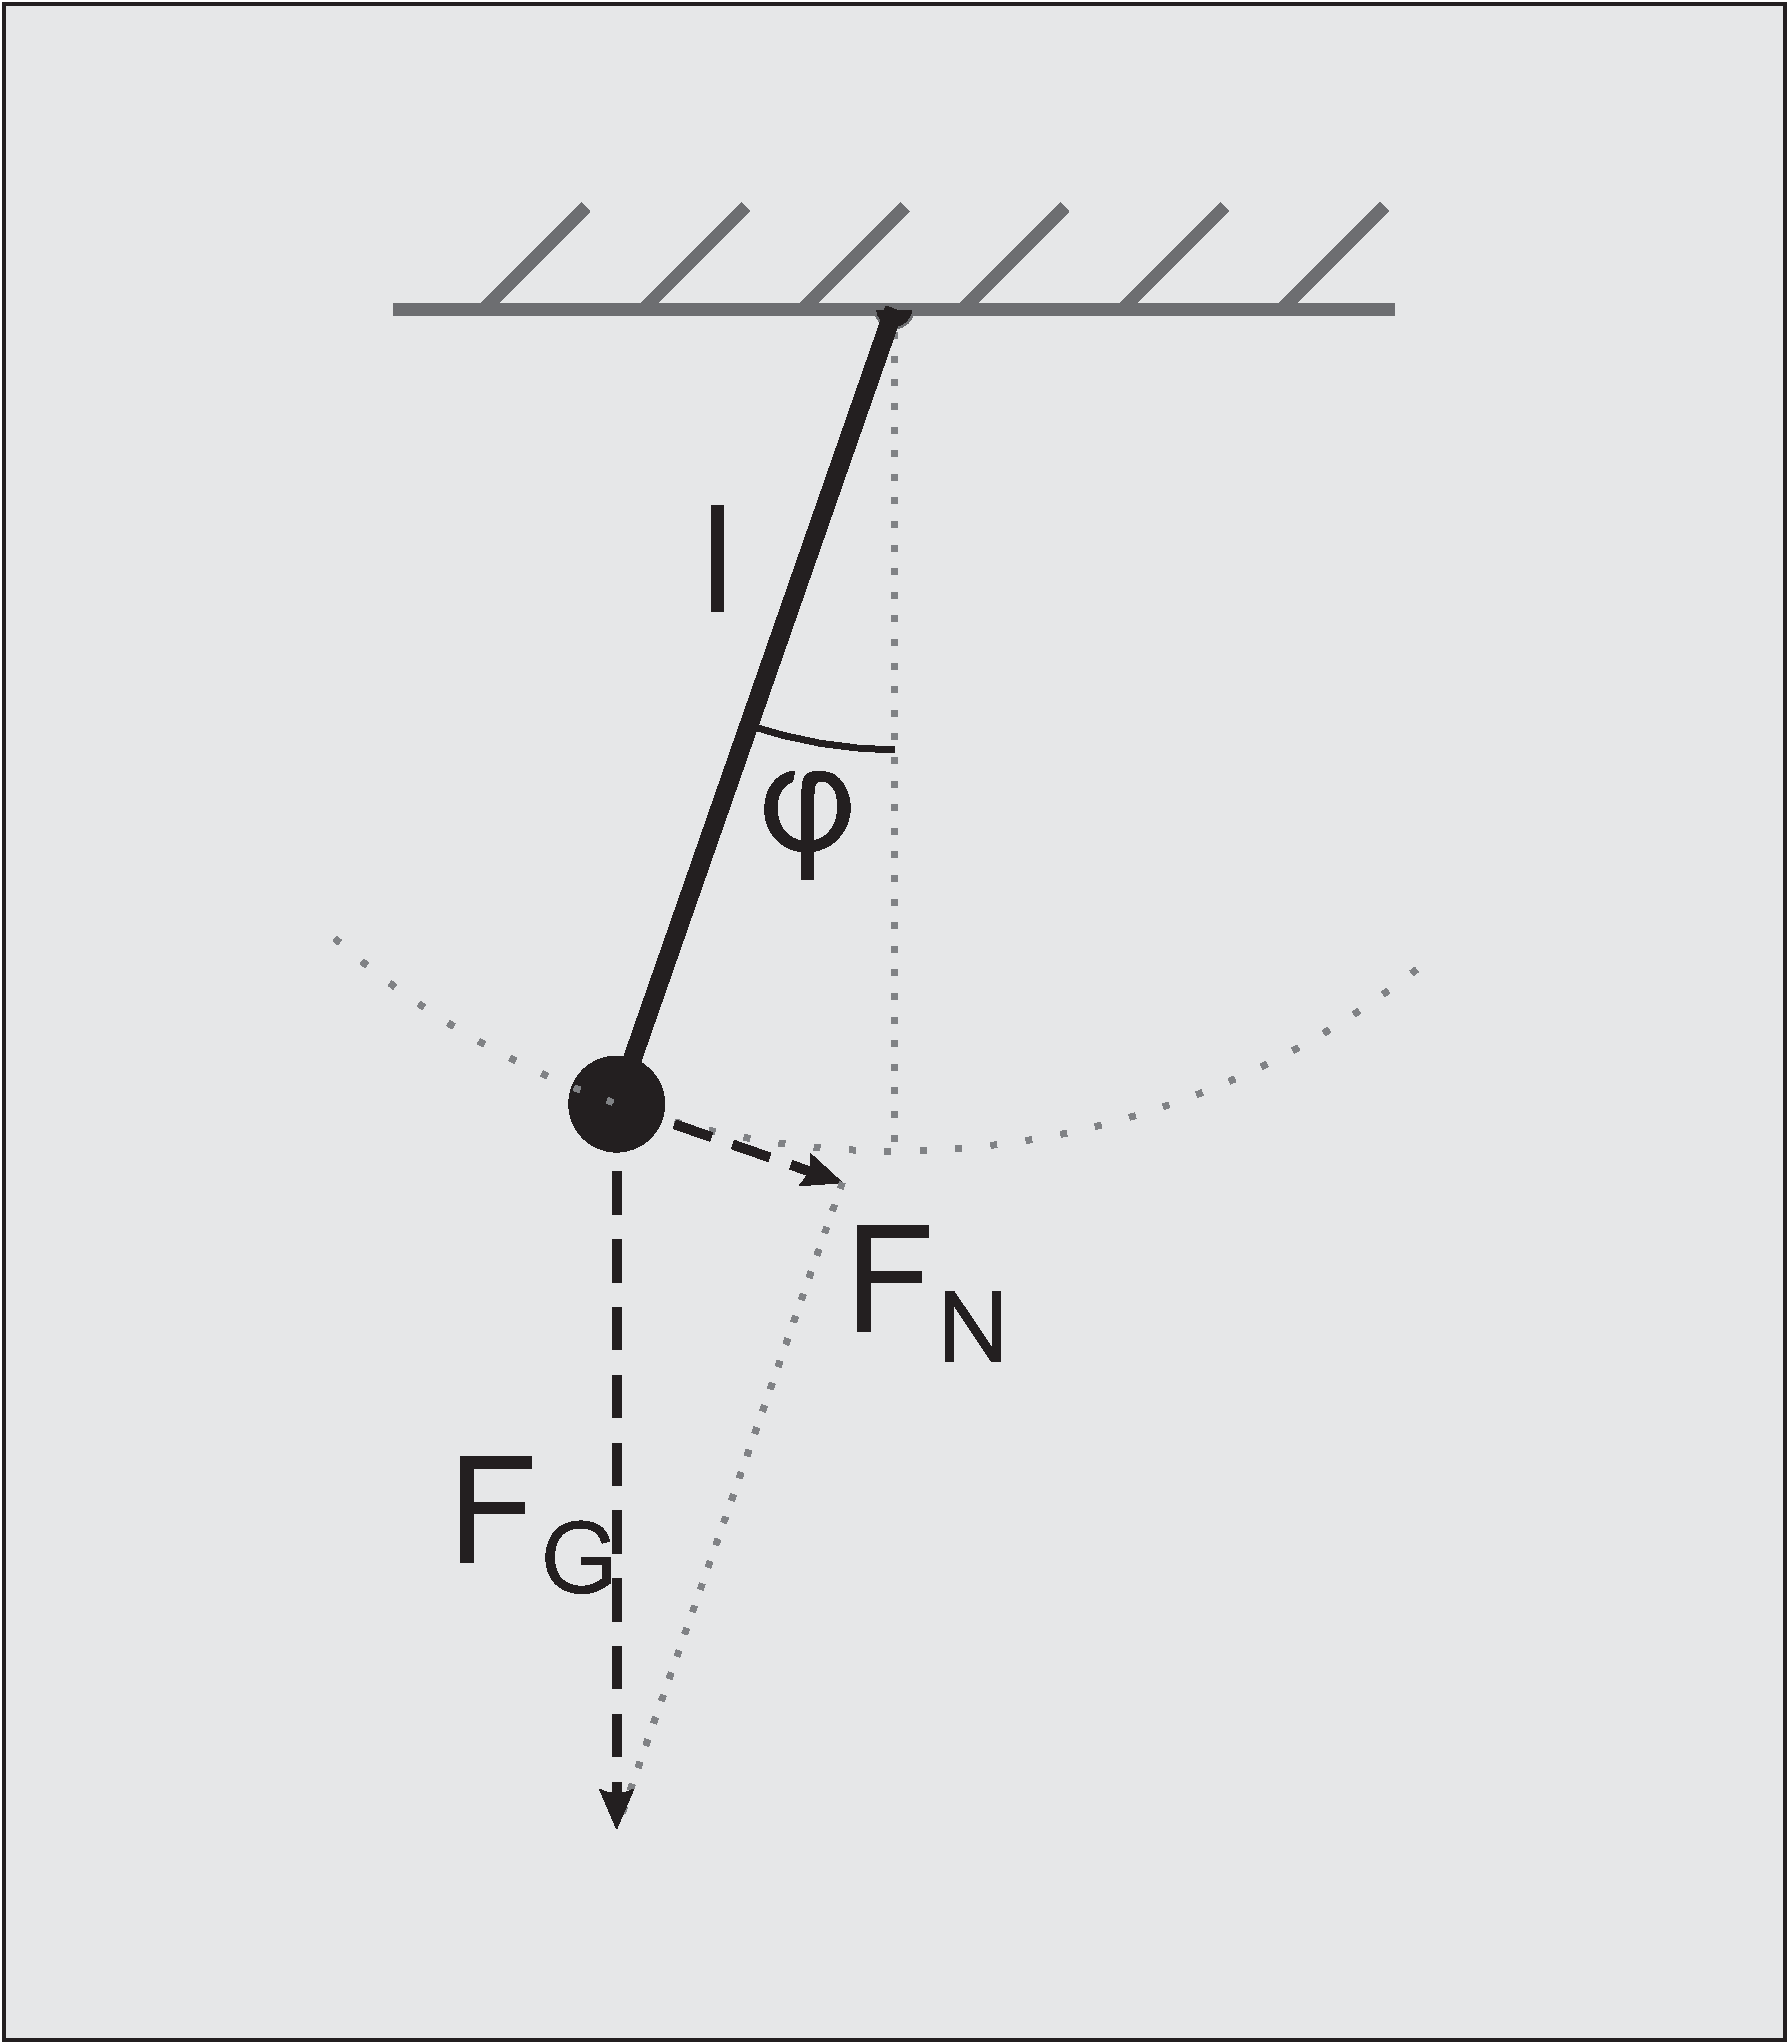
\includegraphics[draft=false,width=1.0\textwidth]{pendulum.pdf}

   \vspace{4ex}
  \end{column}

  \begin{column}{0.65\textwidth}
 \only<1>{
 Newtons law: $m a = F$

 \vspace{2ex}

 Acceleration:  $a = l \ddot{\varphi}$

 \vspace{2ex}

 Force: $F=F_N = - m g \sin \varphi$

 \vspace{4ex}

 $\Longrightarrow$ {\bf ODE for $\varphi$}

 $$\ddot{\varphi} = - g / l \sin \varphi = -\omega_0^2 \sin \varphi$$
 }

 \only<2>
 {

 $$\ddot{\varphi} = - \omega_0^2 \sin \varphi $$

 Small angle: $\sin \varphi \approx \varphi$

 \vspace{2ex}

 Harmonic oscillator $\ddot{\varphi} = - \omega_0^2 \varphi$

 \vspace{2ex}

 Analytic solution: $\varphi = A \cos \omega_0 t + B \sin \omega_0 t$

 \vspace{2ex}

 Determine $A$ and $B$ from initial condition\rem{:

 \centerline{$\varphi(t=0) = \varphi_0 \,\, \text{,} \quad \dot{\varphi}(t=0) = \dot{\varphi}_0$}

 \centerline{$B=\varphi_0 \,\, \text{,} \quad A=\dot{\varphi}_0 / \omega$}}

 }

 \only<3>{

 Full equation: $\ddot{\varphi} = -\omega_0^2 \sin \varphi $

 \vspace{2ex}

 Pendulum with friction and external driving:

 $$\ddot{\varphi} = -\omega_0^2 \sin \varphi - \mu \dot{\varphi} + \varepsilon \sin \omega_E t $$

 \vspace{2ex}

 No analytic solution is known

 \vspace{2ex}

 $\Longrightarrow$ {\bf Solve this equation numerically.}

 }

 \only<4>{

 $$\ddot{\varphi} = -\omega_0^2 \sin \varphi - \mu \dot{\varphi} + \varepsilon \sin \omega_E t $$

 \vspace{2ex}

 Create a first order ODE

 \vspace{1ex}

 \centerline{$x_1 = \varphi \,\, \text{,} \quad x_2 = \dot{\varphi}$}

 \vspace{-3ex}
 \begin{align*}
   \dot{x_1} &= x_2 \\
   \dot{x_2} &= - \omega_0  \sin x_1 - \mu x_2 + \varepsilon \sin \omega_E t  
 \end{align*}


 $x_1$ and $x_2$ are the state space variables

 }
   
  \end{column}
\end{columns}

 

\end{frame}







\begin{frame}[fragile]

\centerline{ \Large Let's solve the pendulum example numerically}

\vspace{2ex}
\begin{lstlisting}
#include <boost/numeric/odeint.hpp>

namespace odeint = boost::numeric::odeint;
\end{lstlisting}

\vspace{2ex}

\centerline{$\dot{x_1} = x_2 \,\,\text{,} \quad \dot{x_2} = - \omega_0 \sin x_1 - \mu x_2 + \varepsilon \sin \omega_E t$}

\vspace{2ex}
\begin{lstlisting}
typedef std::array<double,2> state_type;
\end{lstlisting}

\end{frame}

\begin{frame}[fragile]

\centerline{ \Large Let's solve the pendulum example numerically}

\vspace{2ex}

$\dot{x_1} = x_2$, $\dot{x_2} = - g / l \sin x_1 - \mu x_2 + \varepsilon \sin \omega t$

\vspace{2ex}

\begin{lstlisting}
struct pendulum
{
  double m_mu, m_omega, m_eps;

  pendulum(double mu,double omega,double eps)
  : m_mu(mu),m_omega(omega),m_eps(eps) { }

  void operator()(const state_type &x,state_type &dxdt,double t) const
  {
    dxdt[0] = x[1];
    dxdt[1] = -sin(x[0]) - m_mu * x[1] +
        m_eps * sin(m_omega*t);
  }
};
\end{lstlisting}

\end{frame}

\begin{frame}[fragile]
 \centerline{ \Large Let's solve the pendulum example numerically}

\vspace{2ex}
$\varphi(0) = 1 \,\, \text{,} \quad \dot{\varphi}(0) = 0$
\vspace{2ex}

\begin{lstlisting}
odeint::rk4< state_type > rk4;
pendulum p( 0.1 , 1.05 , 1.5 );

state_type x = {{ 1.0 , 0.0 }};
double t = 0.0;

const double dt = 0.01;
rk4.do_step( p , x , t , dt );
t += dt;
\end{lstlisting}

\vspace{2ex}

$x(0) \mapsto x(\Delta t)$

\end{frame}

\begin{frame}[fragile]
 \centerline{ \Large Let's solve the pendulum example numerically}

\vspace{2ex}


\begin{lstlisting}
std::cout<<t<<" "<< x[0]<<" "<<x[1]<<"\n";
for( size_t i=0 ; i<10 ; ++i )
{
  rk4.do_step( p , x , t , dt );
  t += dt;
  std::cout<<t<<" "<< x[0]<<" "<<x[1]<<"\n";
}
\end{lstlisting}

\vspace{2ex}

$x(0) \mapsto x(\Delta t) \mapsto x(2\Delta t) \mapsto x(3\Delta) \mapsto \dots$

\end{frame}


\begin{frame}[fragile]
 \heading{Simulation}

 \vspace{4ex}

 \centerline{Oscillator: $\mu=0 \,\, \text{,} \quad \omega_E = 0 \,\, \text{,} \quad \varepsilon=0$}

 \vspace{2ex}
 
\centerline{Damped oscillator: $\mu=0.1 \,\, \text{,} \quad \omega_E = 0 \,\, \text{,} \quad \varepsilon=0$}

 \vspace{2ex}

 \centerline{Damped, driven oscillator: $\mu=0.1 \,\, \text{,} \quad \omega_E = 1.05 \,\, \text{,} \quad \varepsilon=1.5$}
\end{frame}

\begin{frame}[fragile]

  \heading{Different Steppers}

  \vspace{2ex}

  \begin{lstlisting}
runge_kutta_fehlberg78< state_type > stepper;
  \end{lstlisting}

  \begin{lstlisting}
runge_kutta_dopri5< state_type > stepper;
  \end{lstlisting}

  but controlled steppers are much better

\end{frame}


\begin{frame}[fragile]
 Controlled steppers

 insert graphic

 \begin{lstlisting}
auto stepper = make_controlled( 1.0e-6 , 1.0e6 ,  odeint::runge_kutta_fehlberg78< state_type >() );
odeint::controlled_step_result res = stepper.try_step( p , x , t , dt );
 \end{lstlisting}

 tries to perform the step and updates $x$, $t$, and $dt$

 it works because runge kutta fehlberg has error estimation

\end{frame}


\begin{frame}[fragile]

Controlled steppers

\begin{lstlisting}
auto stepper = make_controlled( 1.0e-6 , 1.0e6 ,  odeint::runge_kutta_fehlberg78< state_type >() );
while( t < t_end )
{
  odeint::controlled_step_result res = stepper.try_step( p , x , t , dt );
  while( res != odeint::success )
  {
    res = stepper.try_step( p , x , t , dt );
  }
}
\end{lstlisting}

Use integrate functions

\begin{lstlisting}
integrate_adaptive( stepper , x , p , t_start , t_end , dt ); 
integrate_adaptive( stepper , x , p , t_start , t_end , dt , observer );
\end{lstlisting}

\begin{lstlisting}
integrate_adaptive( stepper , p , x , t_start , t_end , dt ,
  std::cout << arg2 << "\t" << arg1[0] << "\t" << arg1[1] << "\n" );
\end{lstlisting}

integrate\_const, integrate\_times, \dots

\end{frame}



\begin{frame}[fragile]

\begin{lstlisting}
integrate_const( stepper , p , x , t , dt , observer );
\end{lstlisting}

problem with controlled stepper

\begin{lstlisting}
integrate_const( make_dense_output( 1.0e-6 , 1.0e-6 , runge_kutta_dopri5< state_type >() ) , p , x , t , dt );
\end{lstlisting}


\end{frame}




\begin{frame}
 More steppers

 implicit, symplectic, predictor-corrector, multistep-methods

 maybe small table
\end{frame}




\begin{frame}
 small summary (kann vielleicht auch wieder weg)
 \begin{itemize}
  \item Very easy example -- harmonic oscillator
  \item Basic features of odeint
  \item Different stepper
  \item Controlled steppers
  \item Dense output steppers
  \item integrate functions
 \end{itemize}

 Now, advanced features

\end{frame}



\begin{frame}
 \heading{extended systems}

 \begin{itemize}
  \item<1->Lattice systems
  \item<2->Discretizations of PDEs
  \item<3->ODEs on Graphs
  \item<4->granular systems
 \end{itemize}

 High-Performance-Computing

 zu jedem Punkt ein Bildchen
 
\end{frame}



\begin{frame}[fragile]
 \heading{Phase oscillator lattices} 

 Any oscillator can be described by one variable, its phase.

 (Bild aus phd Talk)

 Trivial dynamics: $\dot{\varphi}=\omega \varphi$

Vielleicht zusammenfuehren mit der naechsten Folie

\end{frame}




\begin{frame}
 \heading{Phase oscillator lattices} 

 Coupled phase oscillators

 Neurosciences

 Heart dynamics

 Synchronization

 Any weakly perturbed oscillator system

 $\dot{\varphi}_k = \omega_k \varphi_k + q( \varphi_{k+1} , \varphi_k ) + q( \varphi_k , \varphi_{k-1} )$

\end{frame}




\begin{frame}[fragile]
 
 Phase compacton lattices

 $\dot{\varphi}_k = \cos \varphi_{k+1} - \cos \varphi_{k-1}$

 state space contains $N$ variables

 \begin{lstlisting}
typedef std::vector<double> state_type;
 \end{lstlisting}

 Animation with compactons and chaos

 space-time plot for visualization of compactons and chaos

\end{frame}





\begin{frame}[fragile]

Ensemble of phase oscillators

$\dot{\varphi}_k = \omega_k + \sum\limits_l \sin( \varphi_l - \varphi_k )$

Synchronization, all oscillator oscillates with the same frequency

Synchronized state $\varphi_k = \omega_S t + \varphi_{0,k} $

\end{frame}



\begin{frame}[fragile]

Classical implementation

\begin{lstlisting}
typedef std::vector<double> state_type;

struct phase_ensemble
{
    state_type m_omega;
    double m_epsilon;

    phase_ensemble(size_t n,double g=1.0,double epsilon=1.0)
    : m_omega(n,0.0),m_epsilon(epsilon)
    {
        create_frequencies(g);
    }

    void create_frequencies(double g) { ... }

    void operator()(const state_type &x,state_type &dxdt,double t) const
    {
         ...
    }
};
\end{lstlisting}

The ODE has now many parameters, use boost::ref

Vielleicht koennen diese beiden Folien weg

\end{frame}



\begin{frame}[fragile]

\heading{Solving ODEs with CUDA using thrust}

What is Thrust
\begin{quotation}
Thrust is a parallel algorithms library which resembles the C++ Standard Template Library (STL). Thrust's high-level interface greatly enhances developer productivity while enabling performance portability between GPUs and multicore CPUs. Interoperability with established technologies (such as CUDA, TBB and OpenMP) facilitates integration with existing software. Develop high-performance applications rapidly with Thrust!
\end{quotation}



\includegraphics[draft=false,width=0.3\textwidth]{thrust_logo.png}
 

\end{frame}


\begin{frame}[fragile]
 
\heading{Solving ODEs with CUDA using thrust}

Where to use it
\begin{itemize}
 \item Large systems, discretizations of ODE, lattice systems, granular systems, etc.
 \item Parameter studies, integrate many ODEs in parallel with different parameters
 \item Initial value studies, integrate the same ODE with many different initial conditions in parallel
\end{itemize}


\end{frame}



\begin{frame}[fragile]
 \heading{Lorenz system -- Parameter study}

 \begin{equation}
  \dot{x} = \sigma ( y - x ) \quad \quad \dot{y} = R x - y - x z \quad \quad \dot{z} = -b z + x y
 \end{equation}

Standard parameters $\sigma=10$, $R=28$, $b=8/3$ deterministic chaos, butterfly effect

picture of Lorenz system

\end{frame}


\begin{frame}[fragile]
  \heading{Lorenz system -- Parameter study}

Vary $R$ from $0$ to $50$, for which parameters the system is chaotic?

Lyapunov exponents, perturbations of the original system

\end{frame}





\begin{frame}[fragile]

Algebras and operations

Euler method

$ x_i(t+\Delta t) = x_i(t) + \Delta t * f_i(x)$

Algebras perform the iteration over $i$ and operation the elementary addition.

Algebras and operations enter the stepper as template parameters

\begin{lstlisting}
typedef runge_kutta4<state_type,value_type,deriv_type,time_type,
    algebra,operations,resize_policy> stepper; 
\end{lstlisting}

\begin{itemize}
 \item {\tt default\_operations}
 \item {\tt range\_algebra} -- Boost.Ranges
 \item {\tt vector\_space\_algebra} -- Passes the state directly to the operations
 \item {\tt fusion\_algebra} -- For compile time sequences, like $std::tuple< double , double >$
 \item {\tt thrust\_algebra} and {\tt thrust\_algebra} -- for thrust
\end{itemize}

\end{frame}


\begin{frame}[fragile]

Thrust example for Lorenz system,

Implementation of the system function 

\end{frame}











\begin{frame}
 More advanced features, die themen können auch auf mehreren folien zusammengefasst werden
\end{frame}


\begin{frame}
 Boost::ref
\end{frame}

\begin{frame}
 boost::range
\end{frame}

\begin{frame}
 complex state types, vielleicht auch nicht
\end{frame}

\begin{frame}
 arbitrary precision types
\end{frame}

\begin{frame}
 matrices as state types
\end{frame}

\begin{frame}
 graph as state types
\end{frame}

\begin{frame}
 self expanding lattices
\end{frame}








